\documentclass[a4paper,11pt]{article}
\usepackage[utf8]{inputenc}
\usepackage[spanish]{babel}
\usepackage{amsmath}
\usepackage{setspace}
\usepackage[T1]{fontenc}
\usepackage{graphicx}
\usepackage{wrapfig}
\usepackage[usenames,dvipsnames]{xcolor}
\usepackage{fancyvrb}
\usepackage{fancyhdr}
\usepackage[vmargin=1.5cm,top=1.7cm,bottom=1.5cm,left=1.5cm,right=1.5cm]{geometry}
\usepackage{parskip}
\usepackage{arev}
\usepackage{ascii}
\usepackage{cmbright}
% \usepackage[default]{comfortaa}
\setlength{\parindent}{18pt}

% \doublespacing
% \singlespacing
% \setstretch{baselinestretch}
\onehalfspacing


\setlength{\textheight}{249mm}
\setlength{\headheight}{15mm}
\setlength{\footskip}{10mm}

\newcommand{\titulo}{Textos y eventos}
\newcommand{\nombre}{Félix J. Marcelo Wirnitzer}
\newcommand{\email}{{\asciifamily<\color{Brown}fjmarcelo@gmail.com\color{Black}>}}

\pagestyle{fancy}
\lhead{
\includegraphics[width=.07\textwidth]{./ArduinoGranCanaria.png}}
\chead{}
\rhead{\footnotesize\titulo}
\lfoot{\footnotesize\nombre\\\email}
\cfoot{}
\rfoot{\footnotesize\thepage}
\renewcommand{\headrulewidth}{0pt}
\renewcommand{\footrulewidth}{0pt}


%opening
\title{\titulo}
\author{\nombre\\\email}
\date{
\includegraphics[width=.15\textwidth]{./ArduinoGranCanaria.png}}

\begin{document}

\maketitle

% \begin{abstract}
% \end{abstract}

\section{Textos en Processing}

Para escribir un texto en Processing usaremos la función
\begin{center}
\texttt{text(string Texto,float X,float Y\color{gray}{[,float Z]}\color{black})}
\end{center}
que dibuja en pantalla. Muestra la información especificada en el primer párametro de sobre el área de trabajo en la 
posición indicada por los parámetros adicionales. A menos que se indique con la función \texttt{textFont()}, se usará 
una fuente con su tamaño predefinidos. El cambio de color del texto se puede hacer con \texttt{fill()}. De igual forma 
se mostrará el texto de acuerdo con la función \texttt{textAlign()}, permitiéndonos dibujar a la izquierda, a la 
derecha o al centro de las coordenadas.

\vspace{8mm}
%%%%%%%%%%%%%%%%%%%%%%
%      Ejemplo 1     %
%%%%%%%%%%%%%%%%%%%%%%
\mbox{\color{Blue}\begin{minipage}{.55\textwidth}%
        \VerbatimInput[fontsize=\scriptsize,frame=lines,label=Ejemplo 1: Diferentes formatos]{./ejemplo1/ejemplo1.pde}%
\end{minipage}}\hspace{.1\textwidth}
\mbox{\begin{minipage}{\textwidth}%
        
\includegraphics[width=.15\textwidth]{./ejemplo1.png}
\end{minipage}}

\vspace{8mm}
%%%%%%%%%%%%%%%%%%%%%%
%      Ejemplo 2     %
%%%%%%%%%%%%%%%%%%%%%%
\mbox{\color{Blue}\begin{minipage}{.55\textwidth}%
        \VerbatimInput[fontsize=\scriptsize,frame=lines,label=Ejemplo 2: Alejamiento mediante el parámetro %
\texttt{Z}]{./ejemplo2/ejemplo2.pde}%
\end{minipage}}\hspace{.1\textwidth}
\mbox{\begin{minipage}{\textwidth}%
        
\includegraphics[width=.15\textwidth]{./ejemplo2.png} 
\end{minipage}}

\vspace{8mm}
%%%%%%%%%%%%%%%%%%%%%%
%      Ejemplo 3     %
%%%%%%%%%%%%%%%%%%%%%%
\mbox{\color{Blue}\begin{minipage}{.55\textwidth}%
        \VerbatimInput[fontsize=\scriptsize,frame=lines,label=Ejemplo 3: Encerrando un texto en una caja %
\texttt{Z}]{./ejemplo3/ejemplo3.pde}%
\end{minipage}}\hspace{.1\textwidth}
\mbox{\begin{minipage}{\textwidth}%
        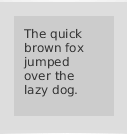
\includegraphics[width=.15\textwidth]{./ejemplo3.png} 
\end{minipage}}

\section{Eventos de teclado y ratón}
Hasta el momento hemos codificado programas solamente secuenciales, es decir, ejecutando línea a línea de principio a 
fin, si bien nos ha servido para los ejemplos es hora de dar un paso mas allá. En esta ocasión veremos lo que son los 
eventos del sistema y como ejecutarlos.

Un evento es una interrupción en el programa principal, ocurre cuando se tiene un cambio externo como por ejemplo 
cuando se presiona una tecla o un clic del mouse. Cuando uno de estos eventos sucede se llama a una función, dentro de 
esta función colocaremos el código a ejecutar.

Las funciones disponibles son las siguientes:
\begin{description}
        \item [\hspace{15mm}\fbox{\ttfamily mouseClicked()}] Ocurre cuando se presiona y se libera un botón del 
ratón.
        \item [\hspace{15mm}\fbox{\ttfamily mousePressed()}] Cuando se presiona un botón del ratón.
        \item [\hspace{15mm}\fbox{\ttfamily mouseDragged()}] Al arrastrar el ratón con un botón pulsado mantenidamente.
        \item [\hspace{15mm}\fbox{\ttfamily mouseReleased()}] En el momento de soltar un botón del ratón que estaba 
presionado.
        \item [\hspace{15mm}\fbox{\ttfamily keyPressed()}] Cuando se pulsa una tecla.
        \item [\hspace{15mm}\fbox{\ttfamily keyReleased()}] En el momento de soltar una tecla presionada.
\end{description}

Para aprovechar al máximo estas funciones se debe hacer uso de las variables del sistema vistas anteriormente, de este 
modo sabremos exactamente qué tecla o botón generó la interrupción.

Las funciones anteriores son del tipo void y no necesitan parámetros para su funcionamiento, veamos un ejemplo para 
comprenderlo mejor:

\vspace{8mm}
%%%%%%%%%%%%%%%%%%%%%%
%      Ejemplo 4     %
%%%%%%%%%%%%%%%%%%%%%%
\mbox{\color{Blue}\begin{minipage}{.55\textwidth}%
        \VerbatimInput[fontsize=\scriptsize,frame=lines,label=Ejemplo 4: Pintando círculos y 
limpiando]{./ejemplo4/ejemplo4.pde}%
\end{minipage}}\hspace{.1\textwidth}
\section{Un ejemplo final}
A continuación un ejemplo que combina las dos partes de este artículo\dots


\mbox{\color{Brown}%
\vspace{5mm}\hspace{1cm}
\begin{minipage}{.65\textwidth}%
\VerbatimInput[fontsize=\scriptsize,frame=lines,label=Ejemplo5: Persiguiendo el texto] 
{./ejemplo5/ejemplo5.pde}%
\end{minipage}}


\end{document}
